%! TEX program = xelatex
% Paquetes:
\documentclass[letterpaper, 12pt]{article}
\usepackage[spanish]{babel} %%Paquete español para mac
\usepackage{graphicx} %% Para incluir figuras
\usepackage{xcolor}
\usepackage{ifpdf}
\DeclareGraphicsExtensions{.pdf}
\usepackage[margin=1in]{geometry}
\setcounter{totalnumber}{5}
\renewcommand{\textfraction}{0.1}
\usepackage[cmex10]{amsmath}
\usepackage{amssymb}
\usepackage{float}
\usepackage{cite}
\bibliographystyle{unsrt}
%\decimalpoint
\usepackage{url}
\usepackage{hyperref}
\hypersetup{colorlinks=false,bookmarksopen=true,linkbordercolor={1 1 1}}
%\usepackage{epstopdf}
\usepackage{mathtools}
\usepackage{chngcntr}
\usepackage{enumitem}
\providecommand{\e}[1]{\ensuremath{\times 10^{#1}}}
\usepackage[parfill]{parskip} % Líneas en lugar de indentación
\usepackage{fancyhdr}
\usepackage{booktabs}
\usepackage{cleveref}
\usepackage{verbatimbox}
\crefformat{footnote}{#2\footnotemark[#1]#3}

\usepackage[squaren]{SIunits} %esto me da nombres de unidades y prefijos
\usepackage{sistyle}% Esto es adecuado para escribir unidades.

\newcommand{\alumno}{Agustín Campeny}
\lhead{\nouppercase{\leftmark}}
\rhead{Tarea 2 - \alumno}
\pagestyle{fancy}
%\usepackage{scrextend}
\numberwithin{equation}{section}

\setlength{\tabcolsep}{6pt} % General space between cols (6pt standard)
\renewcommand{\arraystretch}{0.8} % General space between rows (1 standard)
\begin{document}
\thispagestyle{empty}
%%%%%%%%%%%%%%%%%%%%%%%%%%
%%%%%%%%% ENCABEZADO %%%%%%%%%
%%%%%%%%%%%%%%%%%%%%%%%%%%
\vspace*{-1cm}
\includegraphics[width=2cm]{logo.pdf}
\vspace*{-2.2cm}

\hspace*{2cm}
 \begin{tabular}{l}
  {\ \textsc{\raggedright \footnotesize Pontificia Universidad Católica de Chile}}\\
  {\ \textsc{\raggedright \footnotesize Escuela de Ingeniería}}\\
  {\ \textsc{\raggedright \footnotesize Departamento de Ingeniería Eléctrica}}\\
  {\ \textsc{\raggedright \footnotesize IEE2753 - Diseño de Circuitos Integrados Digitales}}\\
  {\  }\\
 \end{tabular}
 \hfill
\vspace*{-0.2cm}
\begin{center}
  {\Large\bf Tarea 2}\\
\vspace*{2mm}
{\today}\\
\vspace*{2mm}
{\footnotesize \alumno}\\
\vspace*{6mm}
\end{center}
\hrule\vspace*{2pt}\hrule
%%%%%%%%%%%%%%%%%%%%%%%%%%
%%%%%%%%% ENCABEZADO %%%%%
%%%%%%%%%%%%%%%%%%%%%%%%%%

\section{Preguntas cortas}

\begin{enumerate}
  \item ¿Por qué ejecutamos DRC en el diseño? ¿Cómo se relaciona esto con LVS?

    El DRC es un proceso fundamental al utilizar cualquier software CAD para diseñar un dispositivo que luego debe ser fabricado. Este proceso se encarga de analizar el diseño actual, específicamente dimensiones, separaciones, posiciones, densidades, etc, y compararlas con las especificaciones de un proceso de fabricación. Es un método automatizado que asiste en el diseño, y asegura la factibilidad de este al momento de ser enviado a la fabricación.

    El LVS es una sigla para \emph{Layout Vs Schematic}, y es un chequeo automático para verificar si el layout calza efectivamente con lo que se quiere diseñar basado en la planificación, en este caso el esquemático. Tanto DRC como LVS son herramientas automatizadas que asisten y agilizan en el diseño del layout.

  \item Al diseñar el diseño, los NMOS se agrupan y los PMOS se agrupan. ¿Cuál es la razón detrás de esto?

    En la mayoría de los circuitos lógicos CMOS, se busca que la salida de estos sea completamente binaria, es decir o \(V_{DD}\) o \(V_{SS}\), y para lograr esto hay que tener ciertas precauciones con el efecto que tiene el cambio en las entradas. Ya que NMOS y CMOS son complementarios en su funcionamiento, es decir que para una misma entrada se genera el efecto contrario en cada uno (si uno se enciende el otro se apaga), el diseño debe procurar que si un camino se abre hacia uno de los rieles, se cierre el camino hacia el riel opuesto, de lo contrario existe la posibilidad de dejar la salida flotando o de generar una conexión entre rieles (cortocircuito).

    Otro motivo es debido al mecanismo de funcionamiento de los componentes. El criterio de encendido o apagado de los transistores MOS depende del voltaje entre gate y source (\(V_{GS}\)), y del voltaje entre drain y source (\(V_{DS}\)). Un transistor apagado quiere decir que este se encuentra en región de corte, la que se logra cuando \(V_{GS} < V_{Th}\), y un transistor encendido es aquel que se encuentra en región de triodo, lo que se logra cuando \(V_{GS} > V_{Th}\) y \(V_{DS} < V_{GS} - V_{Th}\). Es por este motivo que se busca conectar el terminal source de los NMOS al voltaje más bajo posible (el mas alto posible en PMOS), y de esta forma asegurar un comportamiento predecible con respecto a su voltaje en gate, y evitar que entre en región activa (mucha disipación de potencia).

  \item Hemos dicho que enrute cada capa de metal en una sola dirección (horizontal o vertical). Explica por qué es una buena idea en diseños grandes y complejos.

    A medida que los circuito se hacen mas densos y complejos, la interconexión entre celdas se hace más complicada y requiere mucho más trabajo por parte del diseñador, o la herramienta de routing. Para facilitar este proceso una buena práctica es mantener una sola dirección para el ruteo en cada capa de metal, y de esta forma es mas sencillo evitar colisiones entre conexiones, al costo de generar rutas menos óptimas y más largas.

  \item Las celdas estándar son puertas que tienen diseños con la misma altura vertical, un riel de tierra que atraviesa la parte inferior de la celda y un riel de alimentación que atraviesa la parte superior de la celda. La ventaja de usar diseños de celdas estándar es que su diseño se puede dividir en filas de celdas estándar y enrutar alimentación / tierra a lo largo del diseño en una cuadrícula. En estos diseños, las filas de celdas alternas se reflejan (voltean verticalmente). ¿Cuál es la ventaja de hacer un diseño como este, en lugar de no reflejar filas alternas?

    La ventaja de invertir verticalmente filas consecutivas es que se puede compartir el mismo riel de alimentación, en lugar de necesitar dos por cada fila, reduciendose de esta manera la altura total del circuito y el área total utilizada.

\end{enumerate}

\section{Compuerta misteriosa}

\begin{enumerate}

  \item El circuito lógico de la figura 1 corresponde a un \emph{Full Adder}. El procedimiento utilizado para determinar esto fue primero la realización de una tabla de verdad, que se presenta a continuación:

    \begin{table}[H]
      \centering
      \begin{tabular}{ccc|cc}
        \(X\) & \(Y\) & \(Z\) & \(F\) & \(G\) \\
        \midrule
        0 & 0 & 0 & 0 & 0 \\
        0 & 0 & 1 & 1 & 0 \\
        0 & 1 & 0 & 1 & 0 \\
        0 & 1 & 1 & 0 & 1 \\
        1 & 0 & 0 & 1 & 0 \\
        1 & 0 & 1 & 0 & 1 \\
        1 & 1 & 0 & 0 & 1 \\
        1 & 1 & 1 & 1 & 1
      \end{tabular}
      \caption{Tabla de verdad de circuito en la figura 1}
    \end{table}

    Se puede notar que las entradas \(X\), \(Y\) corresponden a los sumandos, \(Z\) corresponde al carry in, la salida \(F\) corresponde al resultado  de la suma y \(G\) corresponde al carry out.

  \item Se dibujan los diagramas de palo para la puerta lógica \textbf{XOR} y \textbf{NAND}. Se utiliza el software \emph{xcircuit}, que si bien está hecho para hacer esquemáticos, es también útil para dibujos sencillos. Se utiliza el color azul para representar Metal 1, morado para Metal 2, puntos para contactos entre capas y cuadrados con una equis para los pines de la celda.

    \begin{figure}[H]
      \centering
      \includegraphics[height=280pt]{xor_stick.eps}
      \caption{Diagrama de palo para la puerta XOR}
    \end{figure}

    \begin{figure}[H]
      \centering
      \includegraphics[height=280pt]{nand_stick.eps}
      \caption{Diagrama de palo para la puerta NAND}
    \end{figure}

    Considerando que el alto del sustrato P es de  \(16\lambda\), y del sustrato N es de \(8\lambda\), con los rieles superior e inferior y 6 metales horizontales el alto total de la celda es de \(96\lambda\), asumiendo \(4\lambda\) entre metales y sustratos.

  \item Para el ruteo del circuito completo se utiliza Metal 2 (morado) y Metal 3 (naranjo). La celdas son las mismas del item anterior, pero se le remueven la conexiones internas y se disponen de forma horizontal o vertical para el placement de estas.

    \begin{figure}[H]
      \centering
      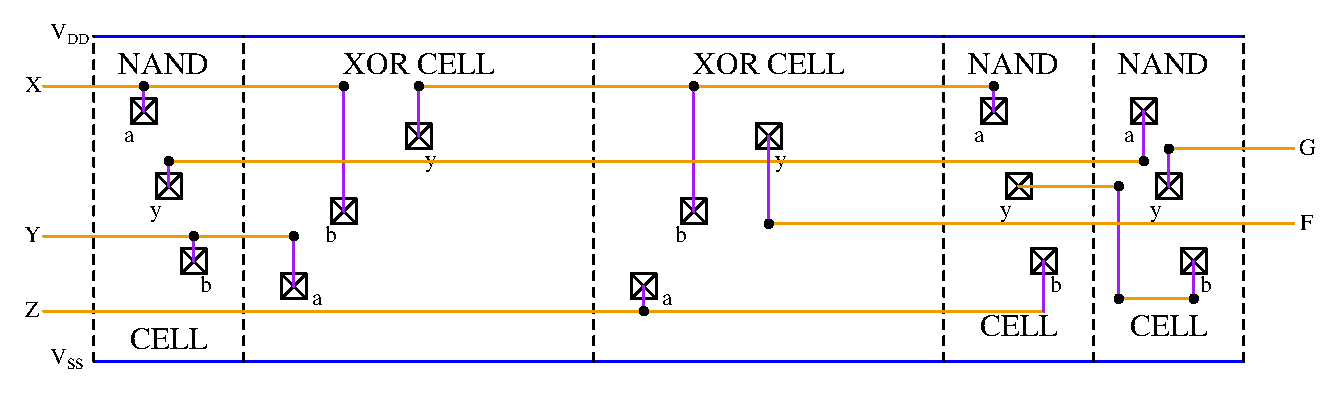
\includegraphics[width=0.9\textwidth]{full_adder.eps}
      \caption{Vista abstracta de circuito completo}
    \end{figure}

  \item Para poder darle mérito al sintetizador y que esta no sea trivial, se implementa un código verilog correspondiente al circuito a nivel de comportamiento, es decir, un full adder combinacional. El modulo fue llamado \texttt{f\_addr} y se encuentra en las carpetas de la tarea junto al verilog sintetizado. A continuación se presenta un bosquejo del resultado de la síntesis.

  \begin{figure}[H]
    \centering
    % XCircuit output "synth_out.tex" for LaTeX input from synth_out.eps
\def\putbox#1#2#3#4{\makebox[0in][l]{\makebox[#1][l]{}\raisebox{\baselineskip}[0in][0in]{\raisebox{#2}[0in][0in]{\scalebox{#3}{#4}}}}}
\def\rightbox#1{\makebox[0in][r]{#1}}
\def\centbox#1{\makebox[0in]{#1}}
\def\topbox#1{\raisebox{-0.60\baselineskip}[0in][0in]{#1}}
\def\midbox#1{\raisebox{-0.20\baselineskip}[0in][0in]{#1}}
   \scalebox{1}{
   \normalsize
   \parbox{5.26562in}{
   \includegraphics[scale=1]{synth_out.eps}\\
   % translate x=768 y=416 scale 0.38
   \putbox{0.06in}{2.06in}{1.20}{$x$}%
   \putbox{0.06in}{0.89in}{1.20}{$y$}%
   \putbox{0.06in}{0.22in}{1.20}{$z$}%
   \putbox{4.97in}{1.89in}{1.20}{$f$}%
   \putbox{4.97in}{0.64in}{1.20}{$g$}%
   } % close 'parbox'
   } % close 'scalebox'
   \vspace{-\baselineskip} % this is not necessary, but looks better

    \caption{Resultado de la síntesis del circuito}
  \end{figure}

  Si bien el circuito resultante no posee la misma implementación que en el enunciado, es un circuito equivalente.

\end{enumerate}

\section{Síntesis}

Se realiza la síntesis de los módulos rtl creados en la tarea 1 utilizando el software libre \emph{yosys}, y las celdas estándar \texttt{osu\_05}, provistas por \emph{Oklahoma State University}. Luego de realizar  la síntesis, se chequea de manera breve si el resultado es consistente con lo esperado con respecto al módulo rtl, y se comenta al respecto.

Se utilizó el siguiente script para yosys:

\begin{verbatim}
# read design
read_verilog ../../rtl/lfsr16/lfsr16.v

# generic synthesis
synth -top lfsr16

# mapping to osu05_stdcells.lib
dfflibmap -liberty osu05_stdcells.lib
abc -liberty osu05_stdcells.lib
clean

# write synthesized design
write_verilog synth.v
\end{verbatim}

\subsection{lbshifter}

La síntesis de este módulo se realizó sin problemas, entregando las siguientes estadísticas:

\begin{verbatim}
=== lbshifter ===

   Number of wires:                  2
   Number of wire bits:             16
   Number of public wires:           2
   Number of public wire bits:      16
   Number of memories:               0
   Number of memory bits:            0
   Number of processes:              0
   Number of cells:                  0
\end{verbatim}

Por como está implementado el módulo, que es simplemente un shift circular hacia la izquierda, solo son necesarios wires para la entrada y salida, sin necesidad de compuertas ni registros.

\subsection{asr8}

La síntesis de este módulo pasó sin problemas, con la siguiente estadística:

\begin{verbatim}
=== asr8 ===

   Number of wires:                119
   Number of wire bits:            194
   Number of public wires:          13
   Number of public wire bits:      88
   Number of memories:               0
   Number of memory bits:            0
   Number of processes:              0
   Number of cells:                178
     $_ANDNOT_                      12
     $_AND_                          1
     $_AOI4_                         8
     $_DFF_PN0_                     64
     $_MUX_                          8
     $_NAND_                         3
     $_NOR_                          1
     $_NOT_                         33
     $_OAI4_                        16
     $_ORNOT_                       10
     $_OR_                          22
\end{verbatim}

Se puede notar que se generaron 64 flip flops, que corresponden a 8 bits por registro por 8 registros que es el valor de largo por defecto. El resto de las celdas forman parte de la logica para el reset de los registros y la salida con respecto al address en la entrada.

\subsection{lfsr16}

El proceso de síntesis se realizó sin problemas, dando la siguiente estadística como resultado:

\begin{verbatim}
=== lfsr16 ===

   Number of wires:                 40
   Number of wire bits:             85
   Number of public wires:           6
   Number of public wire bits:      51
   Number of memories:               0
   Number of memory bits:            0
   Number of processes:              0
   Number of cells:                 51
     $_ANDNOT_                      16
     $_DFFSR_PPP_                   16
     $_NOR_                         16
     $_XNOR_                         2
     $_XOR_                          1
\end{verbatim}

A simple vista la síntesis pareciera haber dado resultados correctos en cuanto al número y tipo de compuertas, apreciándose 16 registros que conforman el shift register. Al revisar el archivo verilog de salida, se puede notar que las compuertas NAND y NOR son utilizadas para asignar el valor del seed al hacer reset, y las compuertas XOR y XNOR son utilizadas en los taps para realizar el feedback. Si bien se esperarían 3 compuertas XOR para que calce con el diseño, utilizar 2 XNOR y 1 XOR es un circuito equivalente.

\subsection{mac8}

Al intentar la síntesis de este módulo, apareció el error \texttt{ERROR: Multiple edge sensitive events found for this signal!} que impidió la síntesis de este. Investigando un poco\footnote{\url{https://www.reddit.com/r/yosys/comments/5cnvzz/error_with_synthesizing_some_verilog_code/}}, se encontró que el siguiente fragmento de código no era sintetizable debido a que el if es gatillado tanto por una señal síncrona como una asíncrona:

\begin{verbatim}
if (~rst || counter >= 7) begin
  counter <= 0;
  accumulator <= 0;
end
\end{verbatim}

La solución fue separar el bloque anterior en un bloque \texttt{if-else if}. A continuación se presenta la estadística de la síntesis:

\begin{verbatim}
=== mac8 ===

   Number of wires:                401
   Number of wire bits:            466
   Number of public wires:           7
   Number of public wire bits:      54
   Number of memories:               0
   Number of memory bits:            0
   Number of processes:              0
   Number of cells:                432
     $_ANDNOT_                      88
     $_AND_                         66
     $_AOI3_                        39
     $_DFF_PN0_                     20
     $_NAND_                        22
     $_NOR_                         21
     $_NOT_                          2
     $_OAI3_                         5
     $_ORNOT_                        6
     $_OR_                          14
     $_XNOR_                        65
     $_XOR_                         84
\end{verbatim}

A simple vista el resultado parece correcto, considerando que hay 20 registros; 16 para el acumulador y 4 para el contador.


\end{document}
